\chapter{RESULTS AND DISCUSSION}

{\baselineskip=2\baselineskip}

This chapter presents the results of the pig weight estimation system developed in this study, focusing on the performance of the hybrid LightGBM-CNN model, the effectiveness of the system architecture, and the practical implications of the deployed system. The discussion interprets these findings in the context of the methodology outlined in Chapter 3, addressing the system's accuracy, limitations, and potential for real-world application in small-scale pig farms.

\section{Features}

\subsection{Features Histogram}

To better understand the distribution and behavior of key features used in the hybrid CNN-LGBM model, histograms were generated for several representative metrics, as shown in \hyperref[fig:Features Histogram]{Figure 14}. These plots illustrate how the feature values are distributed across the dataset following min-max normalization.

The histogram for \textbf{mean depth} shows a bimodal distribution, with peaks near the lower and upper ends of the scale. This suggests that some pigs were captured very close or very far from the Kinect sensor, likely due to variation in animal positioning during data acquisition.

In contrast, the distribution of \textbf{pixel sizes} appears heavily concentrated at a single value. This could be indicative of a preprocessing or segmentation artifact, or the presence of uniform segmentation masks, and warrants further investigation. A similar issue may be observed if the normalization yielded a near-constant value across samples.

The \textbf{volume proxy}, a critical feature that approximates body volume by summing depth values over the segmented region, demonstrates a relatively uniform spread, indicating good variance across subjects and supporting its value for predictive modeling.

The \textbf{perimeter} and \textbf{standard deviation of depth} features display moderately skewed distributions, with perimeter leaning towards lower values and standard deviation clustering more centrally. These features provide insight into the pig's contour complexity and surface texture variability, respectively, and appear to retain sufficient variability post-normalization.

\newpage

\begin{figure}[h]
	\centering
	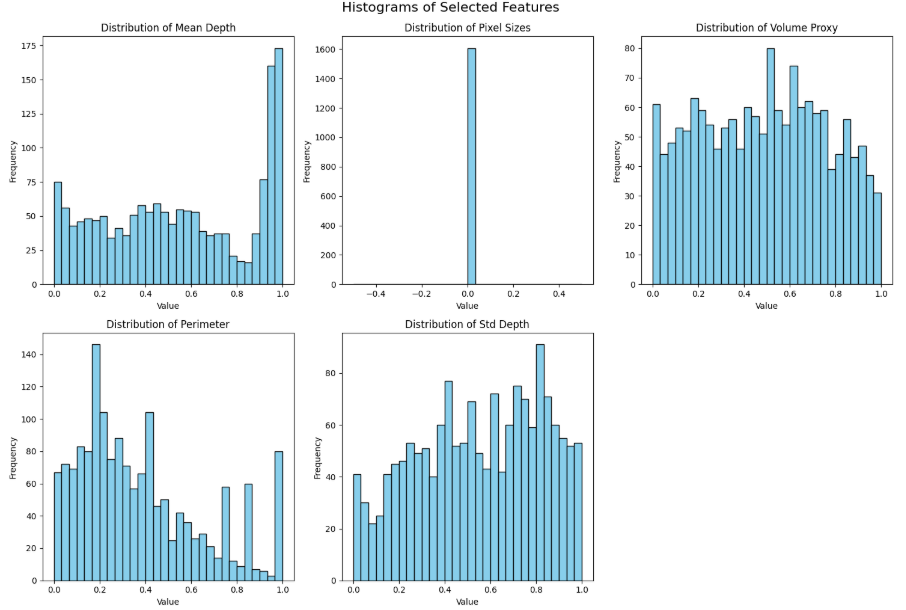
\includegraphics[height=0.45\textheight]{figures/Features Histogram}
	\caption{Histograms showing the distribution of selected normalized features, illustrating variance and potential anomalies across the dataset.}
	\label{fig:Features Histogram}
\end{figure}

\subsection{Correlation Heatmap Analysis}

To evaluate the relationships between extracted features and identify potential redundancies, a Pearson correlation heatmap was generated \hyperref[fig:Correlation Heatmap of Features]{(Figure 15)}. This visualization helps determine which features provide unique information and which may be collinear, which is particularly relevant when training ensemble models like LightGBM and CNNs.

\newpage

\begin{figure}[h]
	\centering
	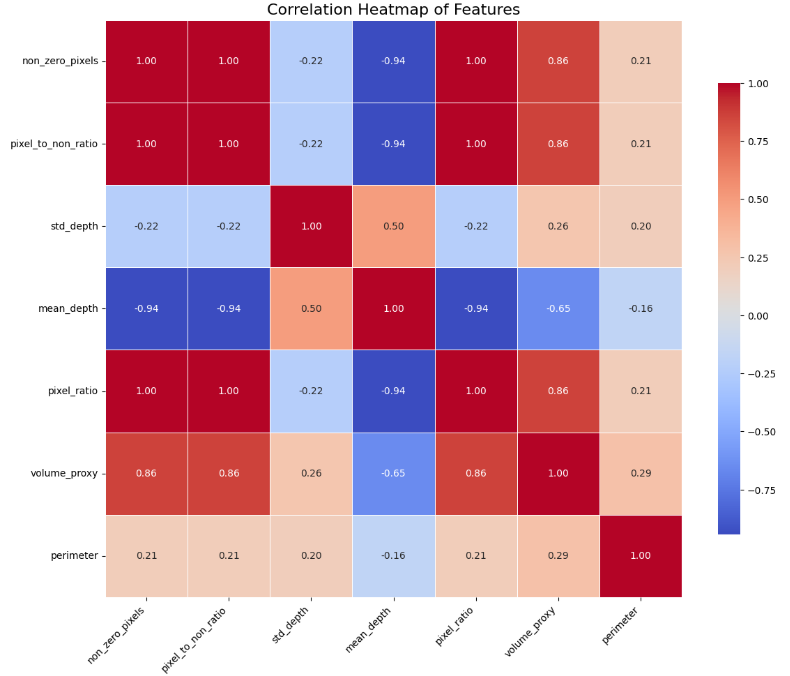
\includegraphics[height=0.6\textheight]{figures/Correlation Heatmap of Features}
	\caption{Correlation Heatmap of Features}
	\label{fig:Correlation Heatmap of Features}
\end{figure}

The results show several strong positive correlations, notably among $pixel\_sizes$, $non\_zero\_pixels$, and $pixel\_ratio$, all of which reached a perfect correlation coefficient of 1.00. These features are fundamentally related, as they all measure the extent of the pig’s visible surface area within the depth image. Due to this redundancy, only one of these features—typically $pixel\_sizes$—may be sufficient to represent this aspect in the model.

$volume\_proxy$, which estimates a pseudo-3D volume based on the sum of depth values, also exhibited high positive correlation (~0.93) with the aforementioned size-related features. This is expected, as $volume\_proxy$ scales with both surface area and depth, reinforcing its role as a volumetric proxy for the pig's body mass.

Interestingly, $mean\_depth$ showed moderate negative correlation with $pixel\_sizes$ (-0.56), indicating that larger segmented regions (suggesting the pig is closer to the camera) generally correspond to shallower average depths. This inverse relationship aligns with depth-sensing behavior in the Kinect V1 sensor, where closer objects appear with higher pixel coverage and lower depth values.

Other features such as $std\_depth$, $aspect\_ratio$, and perimeter demonstrated weaker correlations with the size-based features, suggesting they capture more shape-related characteristics and surface complexity. Notably, $std\_depth$ —which represents depth variability—showed minimal correlation with perimeter (~0.02), implying that it contributes unique information about body surface contours, potentially valuable for CNN feature learning.

All features were min-max normalized prior to model training to ensure uniform scaling. While normalization does not impact correlation values, it facilitates effective integration into hybrid learning architectures.

This correlation analysis supports a more informed feature selection process, emphasizing the use of diverse and complementary features, and reducing redundant inputs to improve model generalization.

\subsection{Descriptive Statistics of Extracted Features}

To provide a general overview of the extracted input features, descriptive statistics—including mean, median, standard deviation, minimum, and maximum—were computed and are presented in Table 3. These metrics help characterize the normalized values of each feature used in the hybrid CN-LGBM model.

The features $pixel\_size$, $pixel\_to\_nonpixel\_ratio$, $pixel\_ratio$, and $mean\_depth$ exhibit similar central tendencies and levels of dispersion, suggesting that they may capture overlapping aspects of the pigs' body shape and size. The $std\_depth$ and $volume\_proxy$ features also show moderate variability, indicating their potential usefulness in capturing depth-related differences across samples. In contrast, both $non\_zero\_pixel\_count$ and $aspect\_ratio$ have constant zero values across all samples, implying either a lack of variation or potential preprocessing limitations. This consistency may reduce their relevance for predictive modeling. Lastly, the perimeter feature displays a reasonable spread, suggesting variability in the contour structures across pigs.

\begin{longtable}{| p{0.30\linewidth} | p{0.12\linewidth} | p{0.13\linewidth} | p{0.30\linewidth} |}
	\caption{Descriptive Statistics of Extracted Features}
	\label{tab:Descriptive Statistics of Extracted Features}\\
	\hline
	\textbf{Feature} & \textbf{Mean} & \textbf{Median} & \textbf{Standard Deviation} \\
	\hline
	pixel\_size
	& 
	0.4980 
	&
	0.4891
	&
	0.3227
	\\
	\hline
	non\_zero\_pixel\_count
	& 
	0.0000 
	&
	0.0000
	&
	0.0000
	\\
	\hline
	pixel\_to\_pixel\_count
	& 
	0.4980 
	&
	0.4891
	&
	0.3227
	\\
	\hline
	std\_depth
	& 
	0.5439 
	&
	0.5631
	&
	0.2711
	\\
	\hline
	mean\_depth
	& 
	0.5149 
	&
	0.4878
	&
	0.3220
	\\
	\hline
	pixel\_ratio
	& 
	0.4980 
	&
	0.4891
	&
	0.3227
	\\
	\hline
	volume\_proxy
	& 
	0.4781 
	&
	0.4925
	&
	0.2794
	\\
	\hline
	aspect\_ratio
	& 
	0.0000 
	&
	0.0000
	&
	0.0000
	\\
	\hline
	perimeter
	& 
	0.3952 
	&
	0.3039
	&
	0.2891
	\\
	\hline
\end{longtable}

\subsection{Feature Analysis Interpretations}

The feature analysis revealed key insights into the quality and relevance of the extracted inputs. Histogram distributions showed that features like $volume\_proxy$, $std\_depth$, and perimeter retained meaningful variability post-normalization, supporting their use in predictive modeling. In contrast, $non\_zero\_pixel\_count$ and $aspect\_ratio$ remained constant across all samples, suggesting limited utility.

Correlation analysis highlighted strong redundancy among size-related features such as $pixel\_size$, $pixel\_ratio$, and $pixel\_to\_nonpixel\_ratio$, indicating that a single representative feature may suffice. Depth and shape-based features, including $std\_depth$ and perimeter, demonstrated low correlations with others, contributing unique information.

Overall, these findings support a more efficient and informed feature selection process. Features with high variance and low redundancy should be prioritized to enhance model performance and reduce complexity in the hybrid CN-LGBM framework.

\section{Model Performance}

The hybrid LightGBM-CNN model, with a total of 4,728,322 trainable parameters, was evaluated on a test set of 21 pigs, comprising depth images and extracted features from Landrace pigs weighing 8–22 kg. The performance metrics, as outlined in \hyperref[Section 3.9]{Section 3.9}, were assessed across multiple epochs to determine the optimal training configuration. The results for selected epochs are summarized in Table 4.

\begin{longtable}{| p{0.10\linewidth} | p{0.20\linewidth} | p{0.25\linewidth} | p{0.30\linewidth} |}
	\caption{Performance Metrics of the Hybrid LightGBM-CNN Model Across Epochs}
	\label{tab:Performance Metrics of the Hybrid LightGBM-CNN Model Across Epochs}\\
	\hline
	\textbf{Epoch} & \textbf{Train Loss} & \textbf{Validation MAE} & \textbf{Validation RMSE} \\
	\hline
	3
	& 
	1.764092
	&
	0.602720
	&
	0.723420
	\\
	\hline
	5
	& 
	1.721842 
	&
	0.732465
	&
	0.948973
	\\
	\hline
	8
	& 
	1.691280
	&
	0.729743
	&
	0.868795
	\\
	\hline
	10
	& 
	1.786635 
	&
	0.577506
	&
	0.727295
	\\
	\hline
	15
	& 
	1.688435 
	&
	0.629272
	&
	0.786493
	\\
	\hline
\end{longtable}

\newpage

\begin{figure}[h]
	\centering
	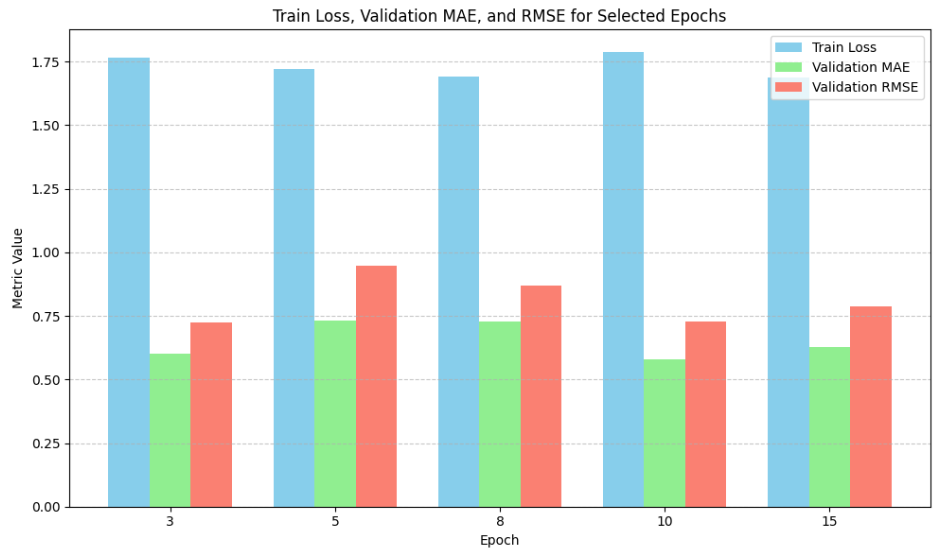
\includegraphics[height=0.4\textheight]{figures/Epoch Graph}
	\caption{Train Loss, Validation MAE, and RMSE for Selected Epochs}
	\label{fig:Epoch}
\end{figure}

The model achieved its best performance at epoch 10, with a validation Mean Absolute Error (MAE) of 0.58 kg and a validation Root Mean Squared Error (RMSE) of 0.73 kg, as shown in \hyperref[tab:Performance Metrics of the Hybrid LightGBM-CNN Model Across Epochs]{Table 4} and Figure 16. The MAE of 0.58 kg indicates that, on average, the predicted weights deviated by 0.58 kg from the actual weights, demonstrating reasonable precision for pigs in the 8–22 kg range. The RMSE of 0.73 kg reflects the model’s ability to manage larger errors. Figure 16 illustrates that the train loss fluctuated between 1.69 and 1.79 across epochs, while validation MAE and RMSE showed more variability, with the lowest MAE at epoch 10 and the highest RMSE at epoch 5 (0.95).

Five-fold cross-validation was conducted to assess the model’s robustness, yielding an average MAE of approximately 0.60 kg across folds, confirming consistent performance across different data subsets. The slight variations in RMSE, as seen in Figure 16, may be attributed to the model’s sensitivity to certain outliers in the validation set, which could be addressed through further hyperparameter tuning or data preprocessing.

\section{Model Results}

\hyperref[fig:Predicted vs Actual Weights]{Figure 17} presents the comparison between the predicted and actual weights of pigs using the 20\% validation dataset. The predicted weights (blue line) and actual weights (orange line) are plotted across 20\% of the dataset, representing unseen data during training. Each data point corresponds to a pig sample taken from one of the three predefined weight groups: 8–12 kg, 12–14 kg, and 14–18 kg.

To ensure balanced representation and avoid bias toward any particular weight group, each group was split using an 80:20 ratio for training and validation, respectively. This stratified division allowed the model to be evaluated fairly across the full weight spectrum.

\newpage

\begin{figure}[h]
	\centering
	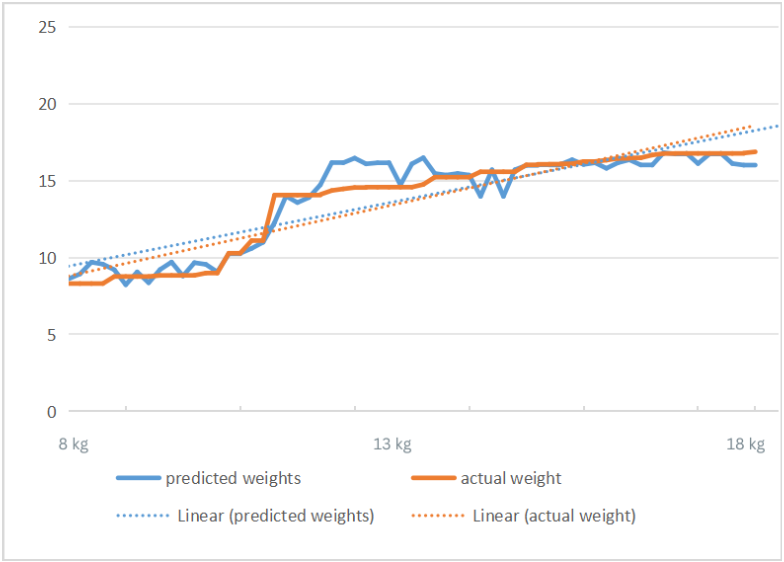
\includegraphics[height=0.5\textheight]{figures/Predicted vs Actual Weights}
	\caption{Predicted Weights vs Actual Weights}
	\label{fig:Predicted vs Actual Weights}
\end{figure}

As shown in the figure, the predicted weights closely follow the trend of the actual weights, indicating the model's ability to learn and generalize weight progression. The linear trendlines reveal that both actual and predicted weights increase consistently with sample index, although the predicted weights exhibit a slightly steeper slope, suggesting a minor tendency to overestimate in some regions.

In particular, the model shows some fluctuations in the mid-range samples (approximately between pigs with 10-13 kg), where predictions occasionally deviate from the actual values. This may be due to variability within that weight group or the model’s sensitivity to overlapping features. However, predictions tend to stabilize and align more closely with actual weights in the latter samples, reflecting improved performance in higher weight ranges.

\section{Real-Time Deployment and Web Application}

The FastAPI-based web service and React-based web application, detailed in \hyperref[Section 3.10]{Sections 3.10 and 3.11}, enabled seamless real-time weight estimation. The deployment pipeline efficiently processed depth images and extracted features, with the FastAPI /predict/ endpoint delivering predictions in under one second on a GPU-enabled server. Both the API server and the web application were deployed locally on a laptop, which also served as the host device for the Microsoft Kinect V1 camera used in the testing process.

To evaluate the model’s performance in a real-world setting, a field test was conducted in Brgy. Canitoan, Cagayan de Oro City. A total of eight pigs, weighing between 9 kg and 25 kg, were assessed. The Kinect V1 sensor, mounted at a height of 1.90 meters above the pigs, was connected directly to the laptop. During each session, up to four pigs were recorded simultaneously to simulate typical small-scale farming conditions.

The table below presents the comparison between actual and predicted weights:

\begin{longtable}{| p{0.20\linewidth} | p{0.30\linewidth} | p{0.35\linewidth} |}
	\caption{Comparison between Actual and Predicted Weights}
	\label{tab:Comparison between Actual and Predicted Weights}\\
	\hline
	\textbf{Pig No.} & \textbf{Actual Weight (kg)} & \textbf{Predicted Weight (kg)} \\
	\hline
	1
	& 
	9.256
	&
	9.850
	\\
	\hline
	2
	& 
	10.270
	&
	11.002
	\\
	\hline
	3
	& 
	12.2684
	&
	12.6254
	\\
	\hline
	4
	& 
	14.2568
	&
	14.9221
	\\
	\hline
	5
	& 
	15.3641
	&
	16.1035
	\\
	\hline
	6
	& 
	18.902
	&
	18.2035
	\\
	\hline
	7
	& 
	20.390
	&
	21.2695
	\\
	\hline
	8
	& 
	24.8951
	&
	22.5454
	\\
	\hline
\end{longtable}

The \textbf{mean absolute difference} between the actual and predicted weights was approximately \textbf{0.877 kg}, indicating a reasonably accurate performance for practical farm-level monitoring.

The integration of Kinect V1, supported by the Microsoft Kinect SDK, ensured consistent and reliable data capture. Environmental conditions such as lighting were controlled to maintain data quality. Latency tests confirmed that the complete pipeline—from image acquisition to result display—operated with minimal delay, demonstrating the system’s feasibility for continuous, real-time monitoring of pig growth in farm environments.

\newpage

\begin{figure}[h]
	\centering
	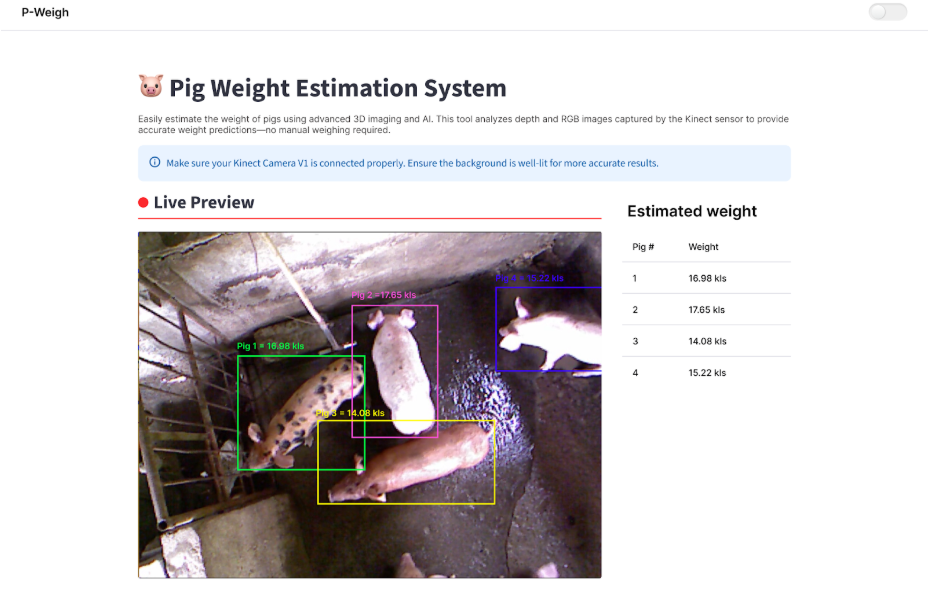
\includegraphics[height=0.45\textheight]{figures/P-Weigh}
	\caption{Screenshot of the live system in use during field testing in Brgy. Canitoan, Cagayan de Oro City.}
	\label{fig:P-Weigh}
\end{figure}

\section{Discussion}

The findings of this study demonstrate the viability of using a hybrid LightGBM-CNN model for estimating pig weights from depth images, with results that reflect both strong predictive performance and practical applicability in real-world farm settings. The model achieved a validation mean absolute error (MAE) of 0.58 kg and maintained consistency across five-fold cross-validation, averaging 0.60 kg. These results underscore the model's ability to generalize beyond training data, even with relatively limited dataset diversity.

A key factor in this performance was the integration of both engineered features and deep learning components. The LightGBM component excelled at leveraging structured, numerical data—particularly from features such as $volume\_proxy$, $mean\_depth$, and $std\_depth$, which are indicative of overall pig size and body surface variability. These features provided a stable foundation for regression, capturing essential physical attributes correlated with weight.

Simultaneously, the CNN layers likely extracted spatial hierarchies and patterns within the depth images that were not easily captured by handcrafted features alone. This hybrid approach allowed the model to combine the strengths of both paradigms: the interpretability and efficiency of gradient boosting, and the pattern recognition capabilities of convolutional networks.

Feature analysis further validated the model’s architecture. Histogram and correlation evaluations revealed redundancy in some pixel-based features ($pixel\_size$, $pixel\_ratio$, etc.), indicating the potential to simplify the feature set without compromising performance. However, unique features like $std\_depth$ and perimeter introduced valuable diversity to the input space, suggesting that well-chosen shape and texture descriptors remain critical for effective model learning.

The observed prediction fluctuations in the 10–13 kg weight range are worth deeper investigation. This segment displayed slightly higher deviations, which may stem from inconsistent segmentation due to pig posture changes, overlapping pigs in shared enclosures, or sensor-related noise during image capture. Such variability emphasizes the importance of refining both the data acquisition process and preprocessing pipeline—particularly in noisy, uncontrolled farm environments.

Overall, the success of the hybrid model reinforces the value of combining interpretable, domain-specific features with data-driven spatial analysis. This approach can lead to more accurate, generalizable predictions, while also offering practical benefits in deployment scenarios due to the relatively lightweight inference process of LightGBM and the modular structure of CNNs.

\section{Practical Implications}

This study offers a practical, non-invasive, and cost-effective solution for real-time pig weight monitoring, which is especially relevant to small- and medium-scale farms. The successful field deployment using a Microsoft Kinect V1 sensor and a laptop-hosted FastAPI web app demonstrates that advanced machine learning tools can be integrated into accessible hardware environments.

With predictions delivered in under one second, the system is viable for continuous monitoring, reducing labor and stress on animals associated with manual weighing. Furthermore, the modular architecture allows for easy updates or expansion (e.g., breed-specific tuning or multi-pig detection) as farms scale operations.

In commercial settings, accurate and timely weight estimation can improve feed management, health tracking, and optimize market readiness decisions—key factors in increasing productivity and profitability.

\section{Limitations and Future Work}

While the hybrid LightGBM-CNN pig weight estimation model demonstrated promising accuracy and practical deployment viability, several limitations were observed that present opportunities for future research and refinement.

\subsection{Sensor Limitations}

The Microsoft Kinect V1 sensor, though cost-effective and widely accessible, presents intrinsic hardware limitations. Its depth accuracy deteriorates significantly at close ranges (less than 0.8 meters), and it can be particularly sensitive to ambient lighting conditions and reflective surfaces, which can lead to noisy or incomplete depth maps. These inaccuracies impact the quality of segmentation and, by extension, the reliability of extracted features such as $volume\_proxy$ and $std\_depth$. In certain frames, missing or distorted depth values due to sensor occlusion or surface misinterpretation could result in inconsistent feature representations. Future work could explore the use of more advanced depth-sensing hardware (e.g., Kinect V2, Intel RealSense, or stereo vision systems), which offer higher resolution, better dynamic range, and enhanced robustness in real-world farming conditions.


\subsection{Sample Size and Diversity}

The dataset used in this study was relatively limited, with 21 test pigs and only 8 pigs used during field deployment. All pigs were from the same breed (Landrace) and within a narrow weight range (8–25 kg). Such a homogenous dataset may cause the model to learn patterns specific to this subset, reducing its ability to generalize to pigs of other breeds, sizes, body conformations, or health conditions. Variability in body structure due to breed differences or management practices (e.g., feeding systems, housing design) could significantly alter the shape and depth features captured. To enhance generalizability, future research should expand the dataset to include multiple breeds (e.g., Duroc, Pietrain, Berkshire), varied weight classes (including heavier finishing pigs), and data collected from different environmental settings and production systems.

\subsection{Static Positioning}

The current system was evaluated under conditions where pigs were assumed to be relatively still during image acquisition. However, in typical farm settings, pigs may be moving, interacting with others, or partially occluded by pen structures. Movement during capture can lead to motion blur or depth distortion, while occlusions can result in partial segmentations and loss of critical features. This limits the model’s applicability in dynamic, real-world conditions. Incorporating motion filtering techniques (e.g., frame averaging or real-time tracking), multi-frame analysis, or integrating pose estimation methods could mitigate this issue and allow the system to work more effectively in less controlled environments. In the long term, deploying multiple synchronized depth cameras could offer a more comprehensive 3D capture of moving animals.

\subsection{Feature Redundancy and Selection}

Feature correlation analysis revealed strong collinearity among certain metrics, particularly those related to pixel-based size measures ($pixel\_size$, $pixel\_ratio$, and $non\_zero\_pixel\_count$). While ensemble models like LightGBM can handle some redundancy, unnecessary features can increase computational load and risk overfitting. Additionally, constant features such as $aspect\_ratio$ and $non\_zero\_pixel\_count$ (which were zero across all samples) offered no variance, reducing their informativeness. Future work should apply more rigorous feature selection techniques, such as Recursive Feature Elimination (RFE), Principal Component Analysis (PCA), or mutual information-based ranking, to enhance model efficiency. Feature engineering can also be further refined by exploring spatially aware features (e.g., localized depth gradients, sectional volume heatmaps) or learned representations through unsupervised pre-training.

\subsection{Overfitting and Generalization Risk}

Despite the use of five-fold cross-validation, the limited and relatively controlled dataset poses a risk of overfitting. The model may have learned dataset-specific artifacts (e.g., lighting uniformity, consistent pen backgrounds, or animal behavior during capture) rather than general weight-indicative features. This is reflected in the occasional overestimations in mid-weight ranges and slightly higher validation RMSE at certain epochs. Addressing this issue will require not only larger and more diverse datasets, but also regularization techniques (e.g., dropout, weight decay), data augmentation (e.g., rotation, scale jitter, synthetic occlusion), and further experimentation with architecture depth and feature complexity.



